\documentclass[12pt]{article}

% log in
% download vs code
% user x64 version
% install
% xxx install vs code wsl extension
% install remote ssh



\usepackage{graphicx}
%\usepackage{subcaption}
\usepackage{amsmath}
\usepackage{amssymb}
%\usepackage{afterpage}
%\usepackage{showlabels}
% \usepackage{epstopdf}
% \usepackage{pdfpages}
\usepackage{geometry}
%\usepackage{wrapfig}
\usepackage{url}
\usepackage{times}
\usepackage{hyperref}
\hypersetup{
    colorlinks=true,
    linkcolor=blue,
    filecolor=magenta,
    urlcolor=cyan,
    pdftitle={Overleaf Example},
    pdfpagemode=FullScreen,
    }

\urlstyle{same}

\newcommand{\soln}[1] {\textit{Solution:} #1}

%\renewcommand{\soln}[1] {}

%\usepackage{cprog}
%\usepackage[compact]{titlesec}
%\titlespacing{\section}{0pt}{5pt}{5pt}
%\titlespacing{\subsection}{0pt}{*0}{*0}
%\titlespacing{\subsubsection}{0pt}{*0}{*0}
%\usepackage[belowskip=-10pt,aboveskip=0pt,margin=10pt,font=footnotesize,labelfont=bf]{caption}

\newcommand{\shortlist}{%
\parindent 0in%
\parskip   0in%
\itemsep   0in%
\topsep    0in%
\parsep    0in%
}

% \setlength{\parskip}{0pt}
% \setlength{\parsep}{0pt}
% \setlength{\headsep}{0pt}
% \setlength{\topskip}{0pt}
% \setlength{\topmargin}{0pt}
% \setlength{\topsep}{0pt}
% \setlength{\columnsep}{0pt}
%\linespread{0.95}

% cost status:
% available: 193,022.87
% liwei (3.5 months): 13555
% me (2 months): 13653
% fringe (13555*.45 + 13653*.079) = 7178
% steve (2 months): 7155
% shujie (2 months): 6700
% total direct: 48241
% total (*1.47): 70914
% available 7/15: 122109

\setlength{\parindent}{0in}

\geometry{letterpaper,tmargin=1in,bmargin=1in,lmargin=1in,rmargin=1in}

%\renewcommand{\normalsize}{\fontsize{11pt}{13.2pt}\selectfont}\normalsize

% \renewcommand{\topfraction}{0.9}	% max fraction of floats at top
% \renewcommand{\bottomfraction}{0.8}	% max fraction of floats at bottom
% % Parameters for TEXT pages (not float pages):
% \setcounter{topnumber}{2}
% \setcounter{bottomnumber}{2}
% \setcounter{totalnumber}{4}     % 2 may work better
% \setcounter{dbltopnumber}{2}    % for 2-column pages
% \renewcommand{\dbltopfraction}{0.9}	% fit big float above 2-col. text
% \renewcommand{\textfraction}{0.07}	% allow minimal text w. figs
% % Parameters for FLOAT pages (not text pages):
% \renewcommand{\floatpagefraction}{0.7}	% require fuller float pages
% % N.B.: floatpagefraction UST be less than topfraction !!
% \renewcommand{\dblfloatpagefraction}{0.7}	% require fuller float pages


%\renewcommand{\familydefault}{\sfdefault}

% TODO
% add figures
% too much?
% look at links (incl comp)
% href
% what to do about points / free choice?

\newcommand{\Title}{PHYS 615 -- HW 1}

\begin{document}

\begin{center}
{\Large\bfseries\Title}

\end{center}
\bigskip
\bigskip

% \begin{tabular}{p{1.7in}p{4in}}
% DOE award number: & DE-SC0006670\\
% Project Title:& Extended MHD modeling of nonlinear instabilities in
% fusion and space plasmas\\
% Project Director /\\ Principal Investigator: & Kai Germaschewski\\
% Date:& 4/15/2015\\
% Period covered:& 4/15/2014 -- 4/15/2015\\
% \end{tabular}

\textbf{Types of homework questions}
\begin{itemize}\shortlist
\item	RQ (Reading questions):  prompt you to go back to the text and read and think about the text more carefully and explain in your own words. While not directly tested in quizzes, can help you think more deeply about quiz questions.
\item	BF (Building foundations):  gives you an opportunity to build and practice foundational skills that you have, presumably, seen before.
\item	TQQ (typical quiz questions):   Similar questions (though perhaps longer or shorter) will be asked on quizzes.  But the difficulty level and skills tested will be similar.
\item Design (D):  These are questions in which you are given a desired outcome and asked to figure out how to make it happen.  These will often also be TQQ’s, but always starting with desired motion/behavior as the given.
\item	COMP (Computing): computing questions often related to TQQ but will never be asked on a quiz (since debugging can take so long).  You will need to do at least four computing questions over the semester
\item	FC (free choice): allows you to decide where to put your time.  Any of the following are possible:  work through a section of the text or a lecture in detail; redo a problem from before; do an unassigned problem in the text; extend a computing project; try a problem using a different analytical approach (e.g. forces instead of conservation of energy).
\end{itemize}

Full credit will be given at 75\% of the total points possible, so you can choose a subset of problems (you can do more / all, but the score is capped at 75\%)

\begin{enumerate}
  \item COMP (10 points)) \textbf{--required--} \textit{Prepare to code}.
  \begin{enumerate}
    \item Decide on a language (Python / Jupyter notebooks is recommended, but Matlab or other options are possible.)
    \item Make sure you have a programming environment that you can work in.
    \begin{itemize}
      \item Jupyter notebooks (though feel free to use another Python environment if you prefer it). Prof. Holtrop's intro to notebooks: \url{https://github.com/mholtrop/phys601/tree/master/Notebooks}
      \item Matlab -- google "UNH matlab student download" to get matlab on your computer
    \end{itemize}
    Hand in code that plots the function $\sin(x)$ for $x$ from $0$ to $2\pi$, using your preferred coding language. All code will be handed in to Canvas, since Gradescope only takes PDF and images, and I want to be able to try out your code.
  \end{enumerate}

\item BF (10 points) \textbf{--required--} \textit{Taylor series.} Look at Equation (2.87) in Taylor (Taylor series). In what way is this expression different from or similar to Taylor series that you have seen in Calculus? What, if anything, is confusing about this equation?

For those of you who do not have the text yet, here is the problem in Taylor:

\centerline{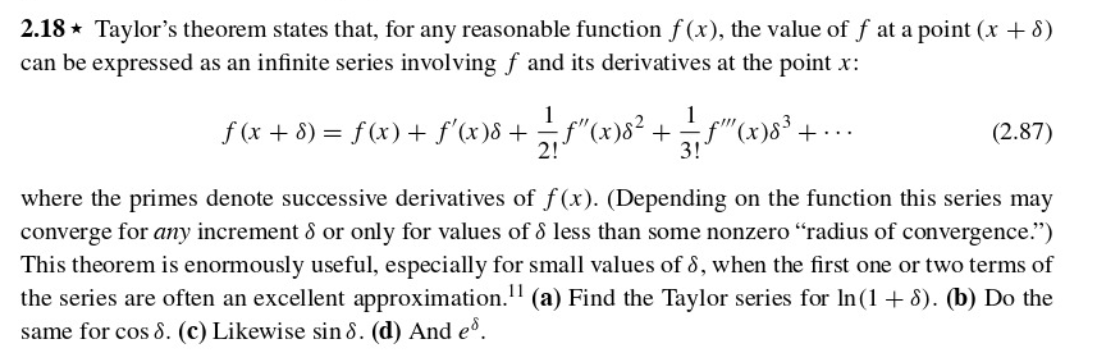
\includegraphics[width=.7\textwidth]{taylor.png}}

\soln{The Taylor series is often written with $f(x)$ on the l.h.s.\ (left hand side), rather than $f(x+\delta)$.

So you may be more familiar with
$$f(x) = f(x_0) + f'(x_0)(x-x_0) + \frac{1}{2} f''(x_0) (x-x_0)^2 + \ldots$$

(Instead of $x_0$, you may see $a$, e.g., in the next problem. Different name, but same thing.) If we take this form and call $\delta \equiv x-x_0$, then $x = x_0 + \delta$, we can substitute that in and get
$$f(x_0 + \delta) = f(x_0) + f'(x_0)\delta + \frac{1}{2} f''(x_0)\delta^2 + \ldots$$

And that is the same as what's written in Taylor, except that he uses $x$ instead of $x_0$. So the way to think about the formula in Taylor is that $x$ is a given fixed value, and $\delta$ is a (typically small) perturbation.
}

\item BF/RQ (10 points) \textit{Taylor series.} Read this page \url{https://www.mathisfun.com/algebra/taylor-series.html} about Taylor series. This is one of many topics that you "should have learned" in previous classes. But getting a deep understanding of math and physics takes significant time and effort. So here is an opportunity to deepen your understanding of this topic.  Here, as in future homework, if you see a topic under “BF” that you are not feeling solid on, I strongly suggest that you do this problem.

\soln{Not a lot to do here. The sigma calculator gives $7.389056098930604$.}

\item	TQQ, D (10 points) \textit{Newton's Law problem.}  This is a modified Atwood machine, with two blocks connected by a massless string over a massless pulley.  Block $A$ rests on a rough horizontal surface with coefficient of static friction $\mu_s$.  What is the maximum mass $m_B$ for $B$ that will allow the blocks to stay motionless?  Give your answer in terms of $m_A$, $g$, and $\mu_s$.  Be sure to check your answer (units, expectations, limiting cases).

\centerline{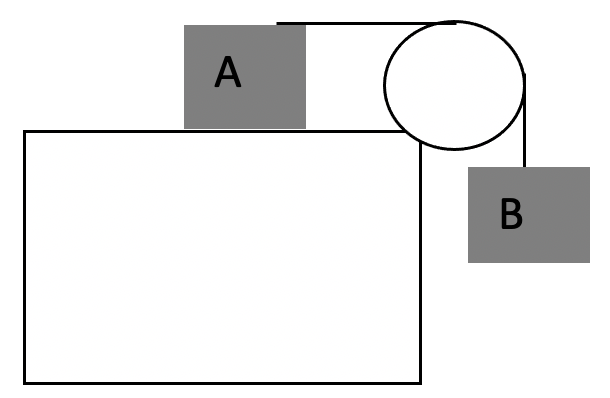
\includegraphics[width=.3\textwidth]{modified_atwood.png}}

\soln{

Since nothing actually moves here, the choice of coordinate system doesn't really matter (acceleration is zero in any direction).

\centerline{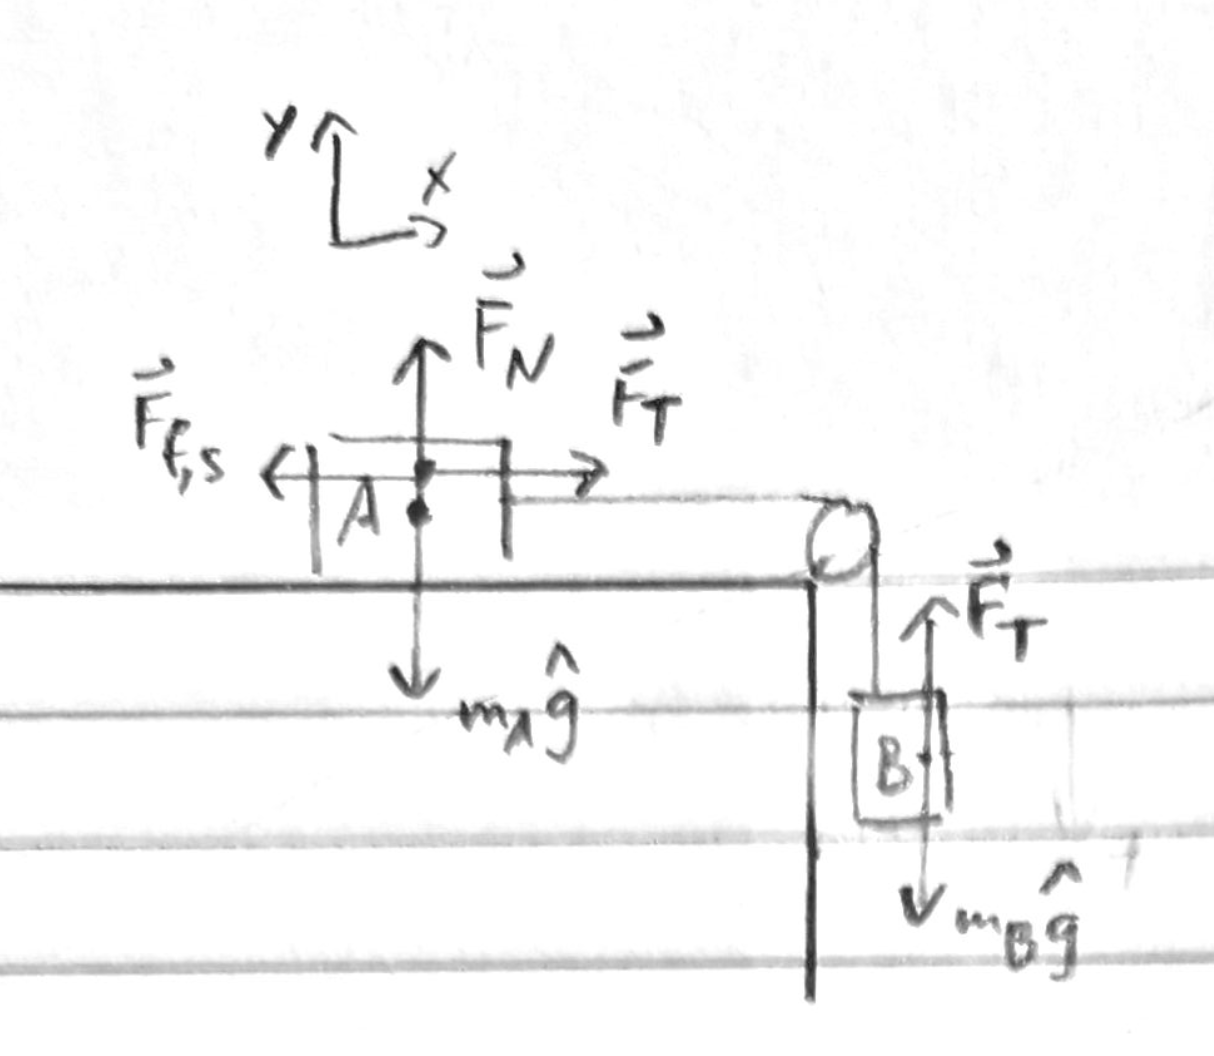
\includegraphics[width=.4\textwidth]{fbd1.png}}

After drawing FBDs, I use Newton's 1st Law (both blocks are and remain at rest), in both $x$ and $y$ for $A$, and just $y$ for $B$:
\begin{align}
  0 &= F_{net, y, on\, A} = F_{N} - m_A g\label{eq:at1}\\
  0 &= F_{net, x, on\, A} = F_T - F_{fs}\label{eq:at2}\\
  0 &= F_{net, y, on\, B} = F_T - m_B g\label{eq:at3}
\end{align}
There is only one relevant normal force, and the tension is the same throughout the string, so I simply used $F_T$ and $F_N$, rather than $F_{T, string\,on\,A}$, etc.

I can use Eqn (\ref{eq:at3})  to solve for $F_T = m_B g$ and substitute that into Eqn (\ref{eq:at2}). I'll also use the formula for static friction. Since I'm looking for the maximum $m_B$, I need as much friction as I can get, ie., the maximum $F_{fs} = \mu_s F_N$. Finally, I can use Eqn (\ref{eq:at1}) to solve for $F_N = m_a g$. Plugging it all in:
\begin{align}
  0 = m_B g - \mu_s m_A g
\end{align}

$g$ cancels out and I find my answer $m_B = \mu_s m_A$.

Checks: Units work out. If I use a heavier block $A$, I can also increase block $B$'s mass without $A$ starting to slide, which makes sense, and if I have rougher (more friction) materials, I can also increase block $B$'s mass. In the limit of no friction, there's less and less $m_B$ I can hold up. :+1:

}

\item TQQ (10 points) \textit{Newton’s Law problem.}  This is a modified Atwood machine, with two blocks connected by a massless string over a massless pulley.  Block $A$ rests on a rough horizontal surface with coefficient of kinetic friction $\mu_k$.  What is the acceleration of the system?  Give your answer in terms of $m_A, m_B, g, \mu_k$.  Be sure to check your answer (units, expectations, limiting cases).

\centerline{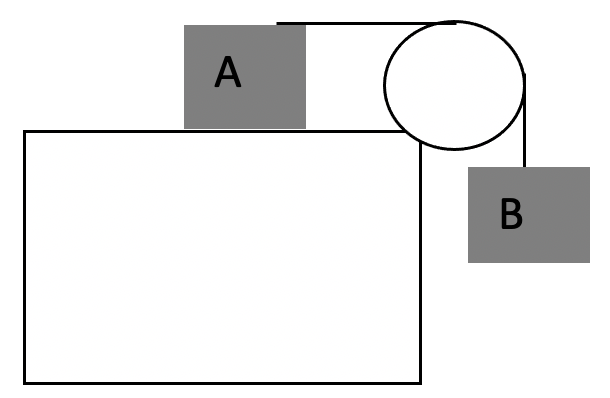
\includegraphics[width=.3\textwidth]{modified_atwood.png}}

\soln{

Now the coordinates matter a bit more.

Since the motion itself is 1-d, I'll make the direction of actual motion positive, that way my acceleration components will be all positive and I'm not in danger of forgetting a minus sign.

I'm going use the usual coordinate system for $A$, that is, $x$ points right, $y$ points up. That way, my acceleration $\vec a_A = a_{A,x} \hat x$, $a_{A_x}$ is positive and hence the magnitude of acceleration is also $a_A = a_{A,x}$. For block $B$, I'll make the direction of motion to be the positive direction as well, ie., down is positive. That way the acceleration of $B$ will be positive as well, and it will equal that of $A$, since $A$ and $B$ are connected by a string of constant length: $B$ moves down just as far as $A$ moves to the right, in the same amount of time, so they always have the same velocity and same acceleration which I will just call $a$.

[It is just as fine to use the "usual" coordinate system everywhere. In that case, one has to be a bit more careful and put in a minus sign, since $B$ is moving down: $a_{A,x} = - a_{B, y}$.]

I will use the same FBD (see above). Since block $A$ is sliding, the force of friction changes to kinetic, and I have to use Newton's 2nd Law since there is acceleration.
\begin{align}
0 &= F_{net, y, on\, A} = F_{N} - m_A g\\
m_A a &= F_{net, x, on\, A} = F_T - F_{fk}\\
m_B a &= F_{net, y, on\, B} = m_B g - F_T
\end{align}

Overall, I have 4 unknowns ($a, F_N, F_T, F_{fk}$), but I also have an additional equation for kinetic friction, so things look promising.

The first equation again gives me my normal force $F_N = m_A g$, which I'll need for the friction $F_{fk} = \mu_k F_N = \mu_k m_A g$.
I'll then add the bottom two equations together, because that way, $F_T$ will drop out:

$$(m_A + m_B) a = m_B g - \mu_k m_A g$$

Solving for $a$:

$$ a = \frac{m_B - \mu_k m_A}{m_A + m_B} g$$

Units work out. A heavier block $B$ will give more acceleration, a heavier block $B$ will reduce acceleration. In the limiting case of no friction, one gets $a = \frac{m_Bg}{m_A + m_B}$, which makes sense since the force of gravity from $B$ accelerates the entire system $m_A + m_B$.

}

\item TQQ, D (20 points) \textit{Newton’s Law problem.}  Block $A$ rests on block $B$, and both slide down an incline with coefficient of kinetic friction $\mu_k$.  The coefficient of static friction between blocks $A$ and $B$ is $\mu_s$. Assume that static friction is large enough to hold Block $A$ still with respect to block $B$.
\begin{enumerate}
  \item	What is the acceleration of the system?
\item	How big must $\mu_s$ be to keep block $A$ still with respect to block $B$?
\item	How big are all of the normal forces?
\end{enumerate}
 Give your answers in terms of $m_A, m_B, g, \mu_k$.  Be sure to check your answer (units, expectations, limiting cases).  Hint:  Example 1.1 in the book reminds you how to work with inclined planes.

 \soln{
  For part a), since we presumably have enough static friction to keep the blocks still relative to each other, I might just as well consider them to be glued together, ie., one big block with mass $M = m_A + m_B$. I can then exactly follow Taylor Ex 1.1 and I'm not going to repeat this here (but you should), ending up with
\begin{align}
a = (\sin\theta - \mu_k\cos\theta) g
\end{align}

For part b), since the static friction is between the two blocks, I now need to look at at least one of them individually. I'll do that for block $B$:

\centerline{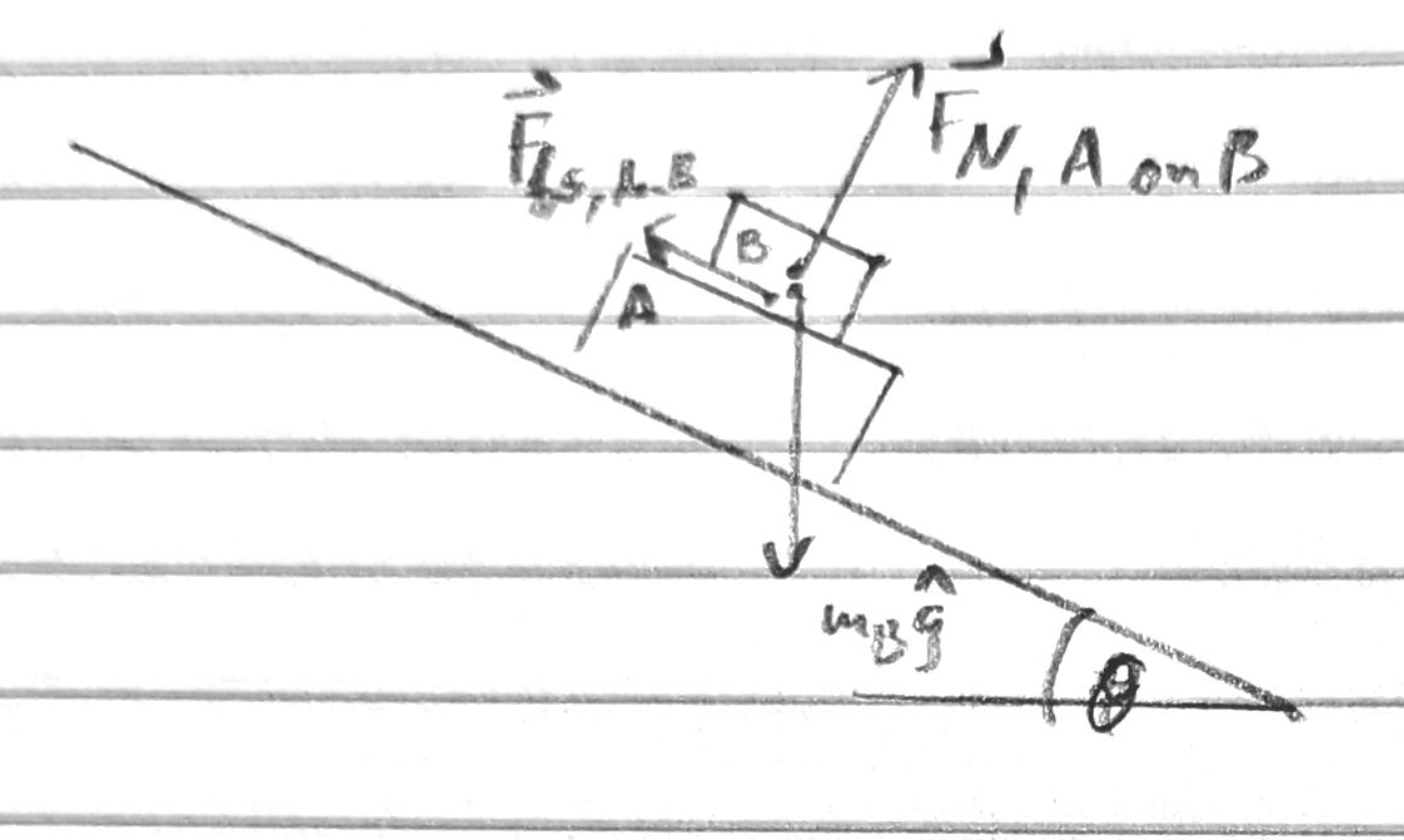
\includegraphics[width=.4\textwidth]{fbd2.png}}

The solution process is actually quite similar. In the normal direction ($y$), the net force has to be 0, and in the direction down the plane ($x$), the net force has to make block $B$ accelerate at the same rate $a$ that both $A$ and $B$ are accelerating at, still assuming they don't move relative to each other. That $a$ we just found in the previous part.

\begin{align}
  0 &= F_{N,A \,on\,B} - m_B g \sin\theta\\
  m_B a &= m_B g \cos\theta - F_{fs, A \,on\, B}
\end{align}

We're looking for the $mu_s$ that's just enough to give us enough friction, ie., $F_{fs, A\,on\,B} = \mu_s F_{N, A\,on\,B}$. Using the 1st equation to find the normal force and plugging things into the 2nd equation, we get:

\begin{align}
m_B (\sin\theta - \mu_k\cos\theta) g = m_B g \cos \theta - \mu_s m_B g \sin\theta
\end{align}

This conveniently simplifies to $\mu_s = \mu_k$.

Besides the units (or lack thereof) checking out, this does make sense: The kinetic friction makes the combination of the two block slow down compared to how they would otherwise accelerate. If there was no friction between $A$ and $B$, then $B$ itself would accelerate at the no-friction rate, which is that same faster no-friction acceleration. If it did that, it would slide down faster than $A$, and slide off of $B$. In order to slow down $B$ to go as fast as the glued together $A-B$ blocks were going it again requires friction, it's just that this time it's static friction since block $A$ is acclerating just as fast.

Note that it is possible for $\mu_s > \mu_k$. That would give static friction more ability to hold together than $A$ and $B$ than what's actually needed. But static friction automatically adjust to be as strong as needed to keep things from starting to slide relative to each other, but no more than needed. (But it can only do so up to a maximum, that is, $mu_s F_N$).

For part c), we (or rather Taylor) found the normal force between block $A$ and the plane to be $(m_A + m_B) g \sin\theta$.
We found the normal force of $A$ on $B$ above to be $m_B g \sin\theta$, and the normal force between $B$ and $A$ is its third law pair, ie., the same (magnitude).

I did not draw a F.B.D. for $A$ by itself, this certainly could be done, and it would involve gravity, two normal forces, and two friction forces. It would be a nice confirmation that everything we already know is consistent, ie., the forces in the normal direction will add up to zero, and the forces in the down-the-plane directions come out to be $m_B a$.

}

%  \item	TQQ (5 points) We discussed in class that the normal force is not always equal the weight of the object.  Give one situation where weight and normal forces are equal, one where the normal force is greater, and one where the normal force is less.  Justify your ranking of the forces by using Newton’s second law and a free body diagram for each situation.

% \item	TQQ (5 points) Complete the table on forces (posted on Canvas/Modules/Forces.overview.pdf) to review how you can tell if a force is acting, how you determine its magnitude and direction.  Feel free to review an intro physics text and if you don’t have one, google “University Physics Open Stax” for access.

\item	TQQ (10 points) Consider a hand, pressed against vertical book $A$, which is in turn pressed against vertical book $B$, which is in turn pressed against a vertical wall; the books are at rest.  There is static friction between all surfaces.  Draw the free body diagrams for books $A$ and $B$.  State in words what the third law pairs are for each force on those books.

\centerline{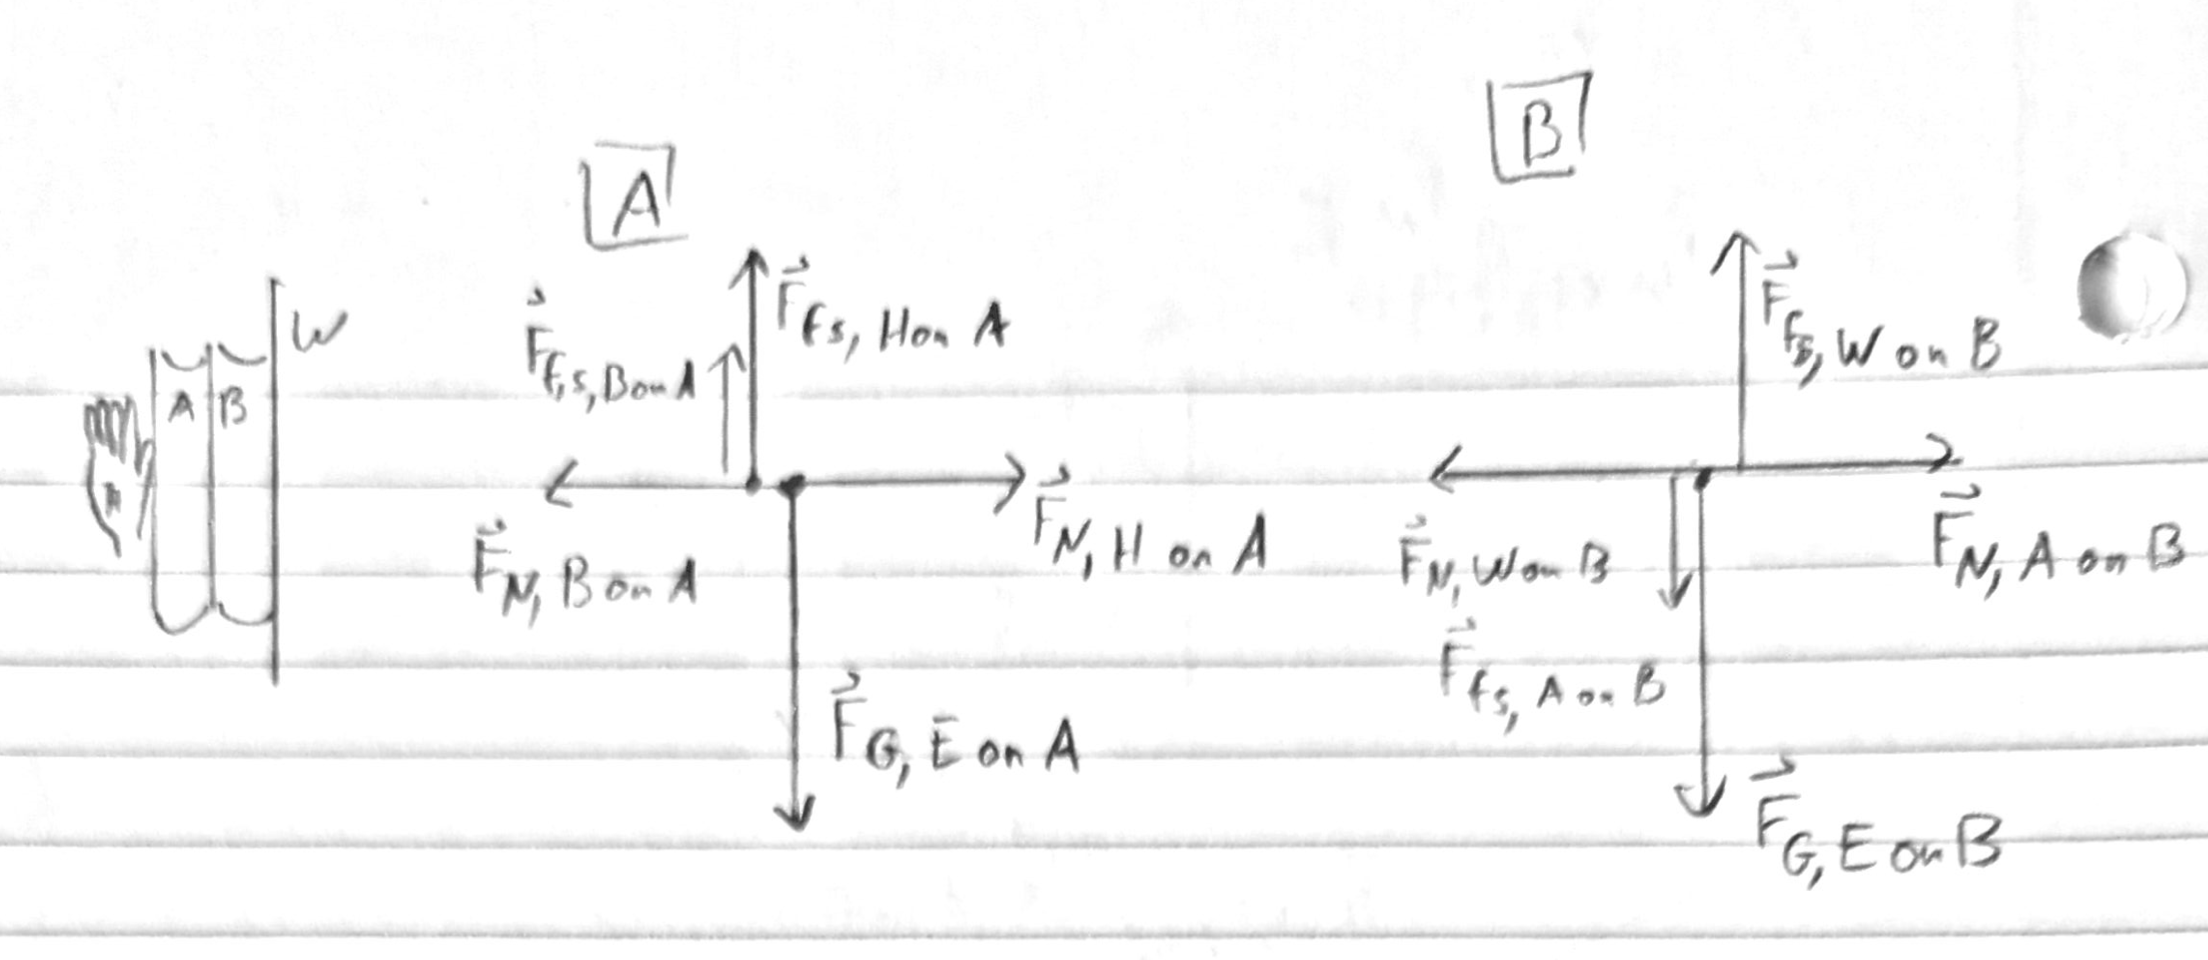
\includegraphics[width=.8\textwidth]{fbd3.png}}

Third-law pairs: $\vec F_{N,B\,on\,A} = -\vec F_{N,A\,on\,B}$, $\vec F_{fs,B\,on\,A} = -\vec F_{fs,A\,on\,B}$, $\vec F_{N,H\,on\,A} = -\vec F_{N,A\,on\,W}$, $\vec F_{N,W\,on\,B} = -\vec F_{N,B\,on\,W}$, $\vec F_{fs,H\,on\,A} = -\vec F_{fs,A\,on\,H}$, $\vec F_{fs,W\,on\,B} = -\vec F_{fs,B\,on\,W}$, $\vec F_{G,E\,on\,A} = -\vec F_{G,A\,on\,E}$, $\vec F_{G,E\,on\,B} = -\vec F_{G,B\,on\,E}$.

The direction for the friction between $A$ and $B$ is not clear given what's known (could be zero, too, but those two are third law pairs, so whatever they are, they have to be equal and opposite).

\item	TQQ (10 points) One argument against Newton’s Third Law, is that if forces are equal and opposite, then forces will always be balanced and there is no motion.  Take a particular simple situation (e.g., a hand accelerating a block on a rough table), draw the free body diagram of the block, identify all third law pairs to the forces acting on the block, and explain why this concern is unfounded.

\soln{It is of course true that Third Law pair forces are equal and opposite, so if one adds them up, they cancel. However, where we typically add them up is to get the net force. The net force on some arbitrary object $A$ is the sum of forces that act on $A$, say including some force $\vec F_{kind, B\,on\,A}$. The third law pair is $-\vec F_{kind, A\,on\,B}$. As such, that third law pair would go into finding the net force on $B$, but it doesn't go into the net force on $A$, so it can't cancel things there.

[If objects $A$ and $B$ are moving together, though, it sometimes makes sense to find the total net force, though. For $A$ and $B$ individually, Newton's 2nd Law holds:
\begin{align}
  m_A \vec a_A = \vec F_{net, \,on\, A}\\
  m_B \vec a_B = \vec F_{net, \,on\, B}
\end{align}

Since both equations are true, one can always add them together. Doing so typically makes sense if one knows that $\vec a_A = \vec a_B = \vec a$. Then one gets $(m_A + m_B) \vec a = \vec F_{net, \,on\, A} + \vec F_{net, \,on\, B}$. In this case, third law pairs between $A$, $B$, ie., internal forces, do in fact cancel out, and that we'll see again when we look at conservation of momentum.


}

\item	FC (10 points) (free choice): allows you to decide where to put your time.  Any of the following are possible: work through a section of the text or a lecture in detail; polish up a group work assignment from class; redo a problem from before; do an unassigned problem in the text; extend a computing project; try a problem using a different analytical approach (e.g. forces instead of conservation of energy).

\end{enumerate}

\end{document}
